%!TEX program = xelatex
% 完整编译方法 1 pdflatex -> bibtex -> pdflatex -> pdflatex
% 完整编译方法 2: xelatex -> bibtex -> xelatex -> xelatex
\documentclass[lang=cn,11pt]{elegantpaper}
\usepackage{xcolor}
\usepackage{listings}
\usepackage{makecell}

\title{\href{https://github.com/trifling-mips/trifling-mips}{trifling-mips} : NSCSCC2020设计报告}
\author{武汉大学一队}

% 不需要版本信息,直接注释即可
% \version{0.07}
% 不需要时间信息的话,需要把 \today 删除。
\date{\today}


\begin{document}

\maketitle

\begin{abstract}
本文系2020年“龙芯杯”武汉大学一队的设计报告。其内容主要包括,trifling-mips的cache部分设计与cpu部分设计。
\keywords{trifling-mips, 龙芯杯}
\end{abstract}


\section{cache}
      
\subsection{icache}
\paragraph{}我们设计的icache如图\ref{icache}所示,为3-pipeline icache。在stage 1,由外围电路通过ibus提供所必须的读指令信号。在pipeline 1会在记录读指令请求的同时,读取出对应的tag和下一个cacheline的tag。如果tag命中,则流水线不中断,同时依据下一个cacheline的tag是否hit决定是否发起预取,否则会检查prefetch模块是否hit:如果hit则将预取的cacheline放到icache里面,这时只会stall一个周期;如果没有hit,则进入ICACHE\underline{\hspace{0.5em}}FETCH状态,向prefetch模块发送请求,得到数据后,便放到icache里面,状态机恢复ICACHE\underline{\hspace{0.5em}}IDLE,继续执行后续操作。在pipeline 2会记录命中信息,并且读取出对应的data。在stage 3便使用这些信息多路选择出最后的rddata,设置rddata\underline{\hspace{0.5em}}vld。在pipeline 3进行sync处理,便交给ibus送出结果。icache在测试的时候尚未对inv和flush进行完整的测试,除此外的部分皆已通过ramdom测试,测试结果如表\ref{iexpr}所示,针对sequ\underline{\hspace{0.5em}}rand的情形,maxsequ在25以上添加prefetch有更好的效果。
\begin{lstlisting}[language={[ANSI]C},numbers=left,numberstyle=\tiny,%frame=shadowbox,
	rulesepcolor=\color{red!20!green!20!blue!20},
	keywordstyle=\color{blue!70!black},
	commentstyle=\color{blue!90!},
	basicstyle=\ttfamily]
	interface cpu_ibus_if();
	// control signals
	logic ready;
	// indicate that corresponding stage shall be directly terminated.
	// flush_1 will be '1' whenever flush_2 is '1'.
	// stall shall be '0' whenever flush_2 is '1'.
	logic stall;		// stall signal from icache
	logic flush_1, flush_2, flush_3;
	// read signals
	logic read;			// whether start read req
	logic rddata_vld;	// whether rddata is valid
	phys_t addr;		// read addr
	uint32_t rddata;	// read data
	
	modport master (
	input ready, stall, rddata_vld, rddata,
	output flush_1, flush_2, flush_3, read, addr
	);
	
	modport slave (
	output ready, stall, rddata_vld, rddata,
	input flush_1, flush_2, flush_3, read, addr
	);
	
	endinterface
\end{lstlisting}
\begin{figure}[htbp]
	\centering
	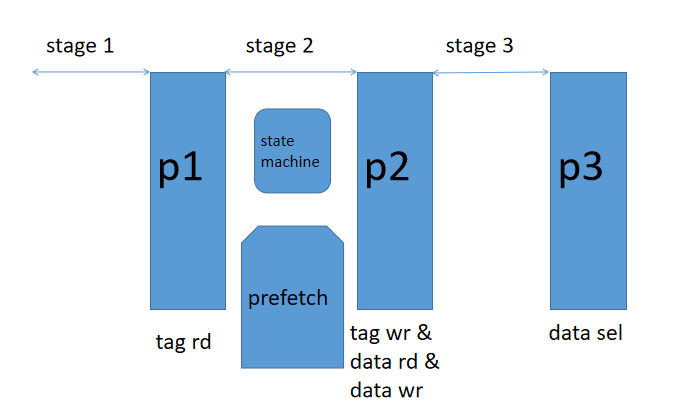
\includegraphics[width=0.6\textwidth]{icache.png}
	\caption{ICACHE 设计}
	\label{icache}
\end{figure}
\begin{table}[h]
	\center
	\caption{icache expr result}
	\label{iexpr}
	\begin{tabular}{|c|c|c|c|c|c|}
		\hline
		n\underline{\hspace{0.5em}}req & with prefetch & sequential(cycle) &  random(cycle) & sequ\underline{\hspace{0.5em}}rand(cycle) & max\underline{\hspace{0.5em}}sequ \\ \hline
		100 & true & 327 & 1320 & 656 & -   \\ \hline
		100 & false & 387 & 1320 & 606 & -   \\ \hline
		1000 & true & 1762 & 10562 & 4625 & 10   \\ \hline
		1000 & false & 2506 & 10393 & 3991 & 10   \\ \hline
		1000 & true & 1762 & 10497 & 2485 & 50   \\ \hline
		1000 & false & 2506 & 10294 & 2869 & 50   \\ \hline
		1000 & true & 1762 & 10500 & 3519 & 20   \\ \hline
		1000 & false & 2506 & 10305 & 3419 & 20   \\ \hline
		1000 & true & 1762 & 10568 & 2798 & 30   \\ \hline
		1000 & false & 2506 & 10360 & 3001 & 30   \\ \hline
		1000 & true & 1762 & 10380 & 2859 & 25   \\ \hline
		1000 & false & 2506 & 10195 & 3045 & 25   \\ \hline
	\end{tabular}
\end{table}

\subsection{dcache}
\paragraph{}我们设计的dcache如图\ref{dcache}所示,为3-pipeline dcache。在stage 1,由外围电路通过dbus提供所必须的lsu\underline{\hspace{0.5em}}req信号。在pipeline 1会在记录req的同时,读取出对应的tag和下一个cacheline的tag。如果tag命中,则流水线不中断,同时依据下一个cacheline的tag是否hit决定是否发起预取,否则会检查write\underline{\hspace{0.5em}}buffer和prefetch模块是否hit:如果write\underline{\hspace{0.5em}}buffer hit且是正在写回或者正在pop则将预取的cacheline放到dcache里面,这时只会stall一个周期,其他情况则依据req直接操作write\underline{\hspace{0.5em}}buffer;如果write\underline{\hspace{0.5em}}buffer没有hit,则检查prefetch是否hit,如果hit则进入DCACHE\underline{\hspace{0.5em}}PREFETCH\underline{\hspace{0.5em}}LOAD状态,这时也只会stall一个周期;如果prefetch没有hit,则进入DCACHE\underline{\hspace{0.5em}}FETCH状态,向prefetch模块发送请求,得到数据后,便放到dcache里面,状态机恢复DCACHE\underline{\hspace{0.5em}}IDLE,继续执行后续操作。在pipeline 2会记录req和读取dcache中的data,这些将在stage 3中使用。stage 3会依据具体的pipeline 2中记录的req决定是写还是读,读操作和icache差不多,写操作会将最新的data与wrdata进行mux,将得到的数据写入到dcache。实验部分(尚未与清华去年的dcache进行对比)如表\ref{dexpr},我们可以发现在官方测试数据集上执行的总周期数cycl和请求数(n\underline{\hspace{0.5em}}req)差别不大,说明4-way lru 16KB的dcache具有较好的性能。
\begin{lstlisting}[language={[ANSI]C},numbers=left,numberstyle=\tiny,%frame=shadowbox,
rulesepcolor=\color{red!20!green!20!blue!20},
keywordstyle=\color{blue!70!black},
commentstyle=\color{blue!90!},
basicstyle=\ttfamily]
typedef struct packed {
logic [$clog2(`N_RESV_LSU):0] lsu_idx;
phys_t addr;		// aligned in 4-bytes
// byteenable[i] corresponds to wrdata[(i + 1) * 8 - 1 : i * 8]
logic [$bits(uint32_t) / $bits(uint8_t) - 1:0] be;
uint32_t wrdata;
logic read, write, uncached;
} lsu_req;
typedef struct packed {
logic [$clog2(`N_RESV_LSU):0] lsu_idx;
uint32_t rddata;
logic rddata_vld;
} lsu_resp;
interface cpu_dbus_if();
// control signals
// for D$
logic stall, inv_dcache;
// for I$
logic inv_icache;
// lsu_req
lsu_req lsu_req;
lsu_resp lsu_resp, lsu_uncached_resp;

modport master (
output inv_dcache, inv_icache, lsu_req,
input stall, lsu_resp, lsu_uncached_resp
);

modport slave (
input inv_dcache, inv_icache, lsu_req,
output stall, lsu_resp, lsu_uncached_resp
);

endinterface
\end{lstlisting}
\begin{figure}[htbp]
	\centering
	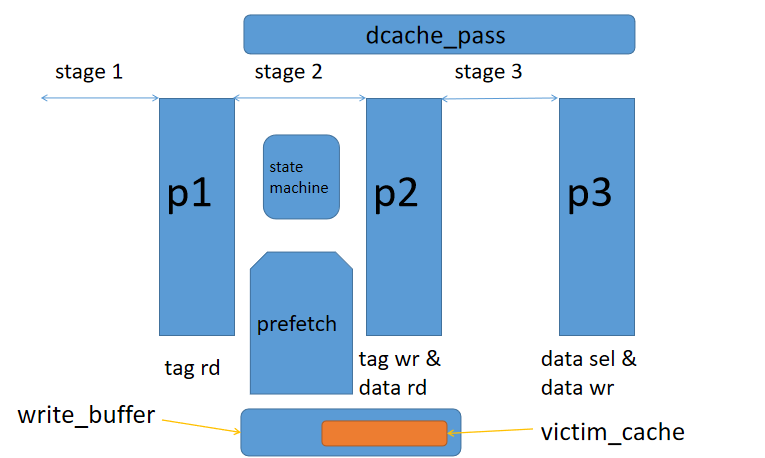
\includegraphics[width=0.6\textwidth]{dcache.png}
	\caption{DCACHE 设计}
	\label{dcache}
\end{figure}
\begin{table}[h]
	\center
	\caption{dcache expr result}
	\label{dexpr}
	\begin{tabular}{|c|c|c|c|c|c|}
		\hline
		name & stall\underline{\hspace{0.5em}}cnt & rd\underline{\hspace{0.5em}}cnt & wr\underline{\hspace{0.5em}}cnt & n\underline{\hspace{0.5em}}req & cycle \\ \hline
		test\underline{\hspace{0.5em}}inv & 7 & 2 & 1 & 6 & 171 \\ \hline
		mem\underline{\hspace{0.5em}}bitcount & 47 & 34 & 0 & 3800 & 4166 \\ \hline
		mem\underline{\hspace{0.5em}}bubble\underline{\hspace{0.5em}}sort & 174 & 118 & 0 & 61613 & 62456 \\ \hline
		mem\underline{\hspace{0.5em}}dc\underline{\hspace{0.5em}}coremark & 142 & 109 & 0 & 82967 & 83677 \\ \hline
		mem\underline{\hspace{0.5em}}quick\underline{\hspace{0.5em}}sort & 778 & 525 & 0 & 38517 & 41704 \\ \hline
		mem\underline{\hspace{0.5em}}select\underline{\hspace{0.5em}}sort & 174 & 118 & 0 & 21594 & 22437 \\ \hline
		mem\underline{\hspace{0.5em}}stream\underline{\hspace{0.5em}}copy & 165 & 91 & 0 & 39924 & 40315 \\ \hline
		mem\underline{\hspace{0.5em}}string\underline{\hspace{0.5em}}search & 303 & 579 & 0 & 33101 & 34525 \\ \hline
		random.2 & 20297 & 6150 & 3932 & 50000 & 161979 \\ \hline
		random.be & 20548 & 6198 & 3951 & 50000 & 162786 \\ \hline
		random & 20805 & 6257 & 4005 & 50000 & 164583 \\ \hline
		sequential & 1024 & 513 & 0 & 32768 & 38531 \\ \hline
		simple & 2 & 2 & 0 & 10 & 152 \\ \hline
	\end{tabular}
\end{table}

\section{cpu}
\subsection{实现的指令集}
实现了初赛要求的57条指令。
\subsection{架构介绍}
单发射五级流水,配备AXI接口。

\end{document}
